\documentclass[12pt,a4paper]{article}
\usepackage[french]{babel}
\usepackage[utf8]{inputenc}
\usepackage[T1]{fontenc}
\usepackage{fancyhdr}
\usepackage{xcolor}
\usepackage{hyperref}
\usepackage{graphicx}
\usepackage{float}
\usepackage{lipsum}
\usepackage{multirow}
\date{01/01/2000}
\usepackage{enumitem}
\setlist[itemize]{label=\textbullet}
\usepackage{amsmath}
\usepackage[colorinlistoftodos]{todonotes}
\usepackage{url}
\usepackage{array}

\title{Le Bug de l'An 2000 : Un Aperçu Complet}

\begin{document}



\begin{titlepage}

\newcommand{\HRule}{\rule{\linewidth}{0.5mm}} 
\center 

\textsc{\LARGE Université de Pau \\ et des Pays de L'Adour}\\[1.5cm] 

\includegraphics[width=7cm, height=4cm]{./images/uppa.png}\\




\HRule \\[0.4cm]
{ \huge \bfseries Le Bug de l'An 2000 : Un Aperçu Complet }\\[0.4cm] 
\HRule \\[1.5cm]


\begin{minipage}{0.4\textwidth}
\begin{flushleft} \large
\emph{Auteurs:}\\
Schneider \textsc{Macxence}\\ 
Giacomoni \textsc{Paul}
\end{flushleft}
\end{minipage}
~
\begin{minipage}{0.4\textwidth}
\begin{flushright} \large
\emph{Professeur:} \\
Manzoor \textsc{Ahmad}
\end{flushright}
\end{minipage}\\[2cm]


01/01/2000\\[1cm]

\textsc{\Large Projet L1 Informatique}\\[0.5cm] 
\textsc{\large UE Latex}\\[0.5cm] 

 

\end{titlepage}


\newpage


\begin{center}
\tableofcontents
\end{center}



\begin{figure}[H]
    \centering
    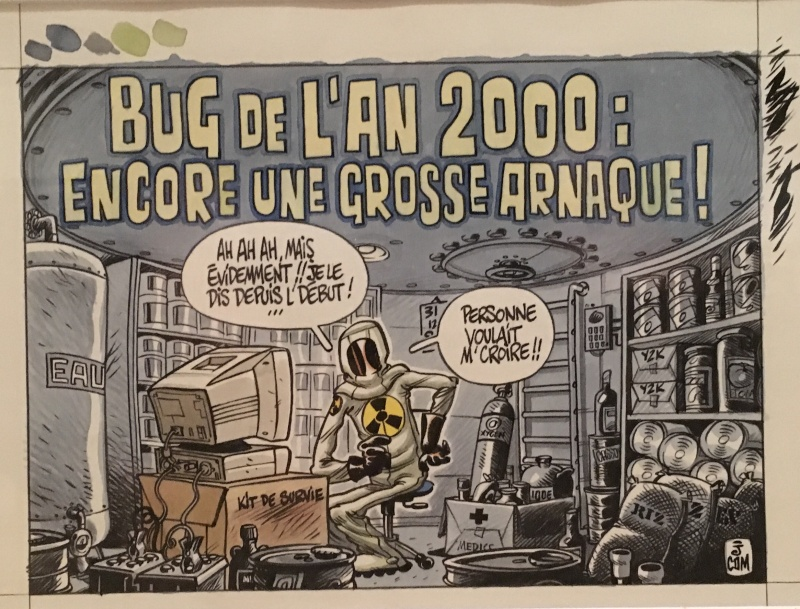
\includegraphics[width=10cm, height=8cm]{./images/bug1.jpg}
    \caption{Bande dessiner : Bug de L'an 2000}
\end{figure}

\newpage
\section{\textit{INTRODUCTION}}
\textbf{Le bug de l'an 2000}, également désigné sous l'acronyme Y2K\footnote{Year 2000}\cite{wik}, est devenu l'un des \textcolor{red}{premiers défis mondiaux de l'ère informatique}, symbolisant à la fois la puissance et les limites de la technologie moderne. À l'aube du 21ème siècle, une question technique apparemment mineure menaçait de déstabiliser des infrastructures informatiques cruciales à travers le monde. Le cœur du problème résidait dans \textit{\textcolor{red}{la façon dont les dates étaient codées dans les systèmes informatiques}}\footnote{exemple : 21/09/99} : par souci d'économie d'espace, seuls les deux derniers chiffres de l'année étaient utilisés pour représenter l'année complète.  \\


L'inquiétude principale résidait dans l'ubiquité des systèmes informatiques dans presque tous les aspects de la vie quotidienne et économique moderne. Des secteurs tels que la banque, l'aéronautique, l'énergie, et même la défense, reposaient sur des logiciels qui auraient pu mal interpréter la date, conduisant à des erreurs de calcul, des pannes de système, et d'autres dysfonctionnements opérationnels. L'urgence de résoudre le bug de l'an 2000 a donc déclenché une course mondiale contre la montre, impliquant une mobilisation sans précédent d'experts en informatique et de ressources financières, dans le but de mettre à jour et de corriger les systèmes vulnérables avant que la nouvelle année ne commence.


\begin{figure}[H]
    \centering
    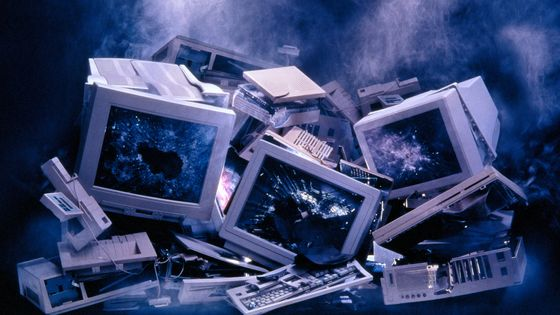
\includegraphics[width=10cm, height=6cm]{./images/bug5.jpg}
    \caption{Image Ordinateur casser}
\end{figure}

\newpage
\section{\textit{Histoire et Origines}}

Pour bien comprendre le bug de l'an 2000, il faut remonter aux débuts de l'informatique. Dans les années 1960 et 1970, \textcolor{red}{ la mémoire était rare et chère\footnote{comme la ram}}. Les programmeurs, pour économiser de l'espace, ont adopté le format de date à deux chiffres\footnote{exemple : 21/09/99}. Cette décision, à l'époque pragmatique, a posé problème des décennies plus tard. Cette pratique, courante et rationnelle à l'époque de son adoption, posait un risque de confusion cataclysmique à l'approche de l'an 2000, car les systèmes informatiques risquaient de ne pas distinguer l'année 2000 de l'année 1900. \\

Les premières alertes datent de la fin des années 1970. Des programmeurs visionnaires ont pointé les risques du format de date abrégé\footnote{De la part des scientifique pour la plupart}. Mais ces avertissements ont été négligés, le problème semblait lointain, et la société n'a pas compris l'ampleur de l'intégration des systèmes informatiques.\\

Dans les années 1990, à l'approche du nouveau millénaire, le bug de l'an 2000 a été pris au sérieux. Les entreprises et les gouvernements ont réalisé que de nombreux systèmes vitaux étaient menacés. Cela a déclenché une vague de mises à jour coûteuses, totalisant des milliards de dollars. Mais l'alternative aurait pu être bien pire.
\cite{ina}

\begin{figure}[htbp]
  \centering
  \begin{minipage}[b]{0.45\textwidth}
    \centering
    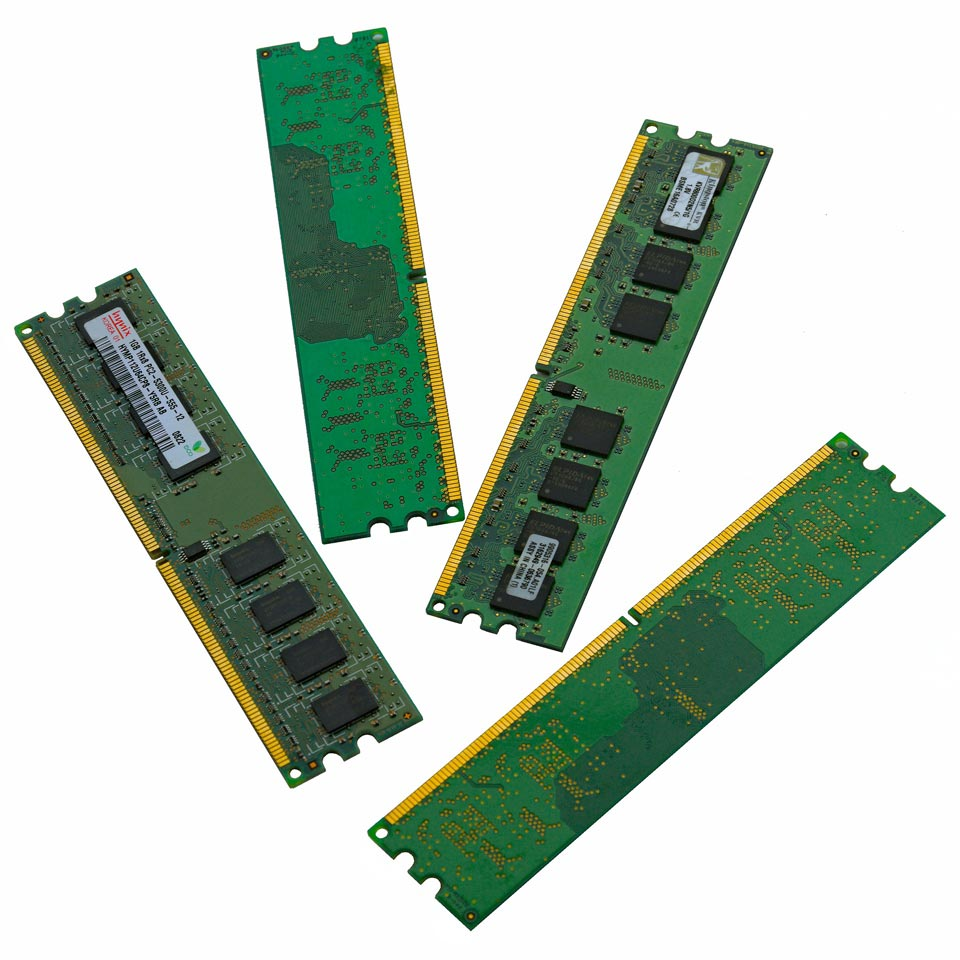
\includegraphics[width=5cm, height=5cm]{./images/ram.jpg}
    \caption{Stockage}
    \label{fig:image1}
  \end{minipage}
  \hfill
  \begin{minipage}[b]{0.45\textwidth}
    \centering
    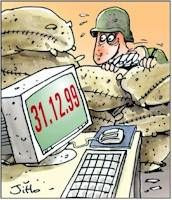
\includegraphics[width=5cm, height=5cm]{./images/bug4.jpg}
    \caption{Passage de 99 à 00}
    \label{fig:image2}
  \end{minipage}
\end{figure}



\newpage
\section{\textit{Impact Potentiel}}
Alors que le 20ème siècle touchait à sa fin, l'ampleur potentielle du bug de l'an 2000 commençait à être pleinement réalisée. Les systèmes informatiques avaient infiltré presque tous les aspects de la vie moderne, de la gestion des infrastructures critiques comme l'énergie et l'eau, à la finance, en passant par les transports et la santé. L'impact potentiel du bug Y2K\cite{y2k} était donc vertigineux, avec des scénarios de pannes électriques généralisées, d'échecs dans les systèmes de contrôle aérien, de perturbations des services bancaires et des marchés financiers, et même de défaillances dans les équipements médicaux critiques. \\

Des études menées à l'époque ont souligné le risque d'une récession économique mondiale si ces systèmes venaient à défaillir simultanément. Les experts ont averti que sans une intervention rapide, le bug pourrait perturber les chaînes d'approvisionnement globales, entraînant une pénurie de biens essentiels, augmentant l'insécurité alimentaire, et potentiellement plongeant de nombreuses régions dans le chaos. Ces perspectives alarmantes ont incité les gouvernements et les entreprises à agir, soulignant la nécessité d'une solution globale et coordonnée. \\
\cite{arcticle}
\begin{center}
Informatique qui commence è prendre une grande place du quotidien :\cite{infoquo}\\

\begin{itemize}
\item Toutes les entreprises on numériser leur quotidien 
\item Nos moyen de payement comme les carte bancaire pouvait être touché 
\item Service de santé / Banque / Transport, numérisé 
\end{itemize}

\end{center}

\begin{table}[H]

\begin{tabular}{|p{2.5cm}|p{2.5cm}|p{2.5cm}|p{2.5cm}|}
\hline
\multicolumn{4}{|c|}{\textbf{\color{red}POTENTIEL IMPACT}} \\
\hline
\textit{ÉCONOMIQUE} & \textit{PUBLIQUE} & \textit{ENTREPRISE} & \textit{COUT} \\ \cline{1-4}
Une Potentiel Crise économique & les services comme les transports, la santé etc. seront forcément touchées & Les entreprises qui ont tout numérisé qui vont avoir des retards & Un cout estimé à plus de 300 milliards de dollars pour pouvoir tout changer \\ \cline{1-4}
\end{tabular}
\caption{Tableau Potentiel Impact du BUG}
\end{table}






\newpage
\section{\textit{Prise de conscience}}

Face à la menace imminente posée par le bug de l'an 2000\cite{bug2000}, une mobilisation mondiale sans précédent a vu le jour. Des milliards de dollars ont été alloués à l'identification, la correction et le test des systèmes informatiques pour garantir leur conformité Y2K\footnote{Year 2000 (rappel)}. Ce processus monumental a impliqué des équipes d'ingénieurs logiciels, des auditeurs de systèmes, et des experts en cybersécurité travaillant sans relâche, souvent 24 heures sur 24, pour examiner des millions de lignes de code à la recherche de la moindre référence non conforme à la date. \\

En plus des efforts de correction logicielle, une importance capitale a été accordée à la sensibilisation et à la préparation des urgences. Les gouvernements ont lancé des campagnes d'information pour préparer le public à d'éventuelles perturbations, tandis que les entreprises ont développé des plans de continuité d'activité pour minimiser les interruptions de service. Cette période a également vu l'émergence de normes et de meilleures pratiques pour la gestion des données et la programmation, qui continuent d'influencer le développement logiciel aujourd'hui.


\begin{figure}[H]
    \centering
    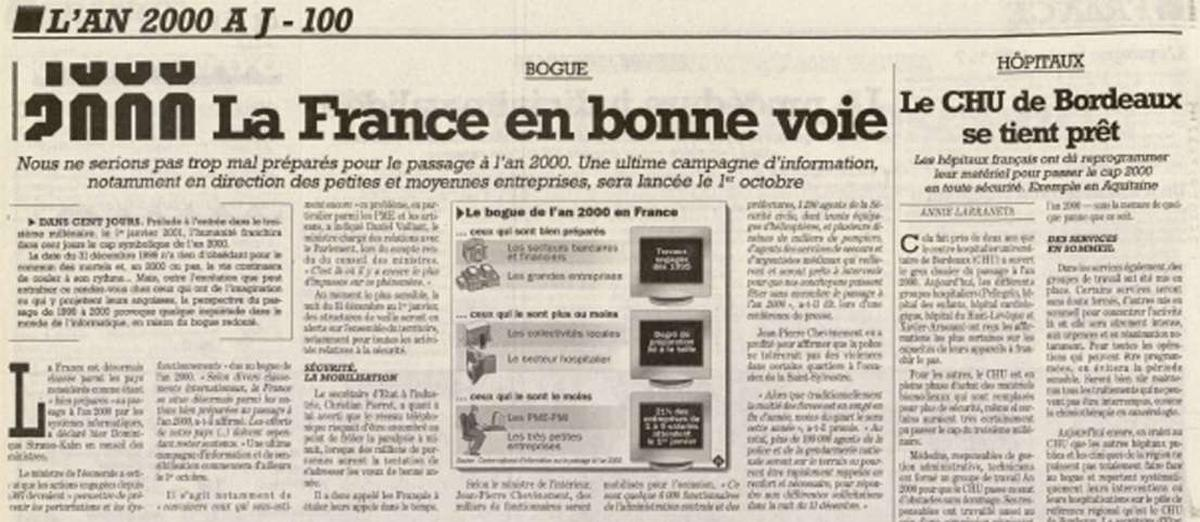
\includegraphics[width=\textwidth]{./images/bug6.jpg}
    \caption{Journal à 100 jours avec le passage à 2000}
\end{figure}



\newpage
\section{\textit{Resultat}}

\subsection{Direct}

Lorsque les horloges du monde entier ont finalement sonné le début du 1er janvier 2000, c'était avec un mélange d'anticipation et d'anxiété. Les célébrations du Nouvel An étaient teintées d'une vigilance prudente, de nombreux yeux étant tournés vers les ordinateurs et les systèmes critiques pour détecter les premiers signes de défaillance. Mais, grâce aux efforts colossaux déployés dans les années précédentes, le passage s'est fait avec remarquablement peu d'incidents majeurs.\\

\begin{center}
\color {red}\textit{" Pour les systèmes informatiques, il vaut mieux investir dans la prévention que de devoir payer le prix fort pour réparer les dégâts " }
\end{center}
\cite{livre}


\begin{figure}[H]
    \centering
    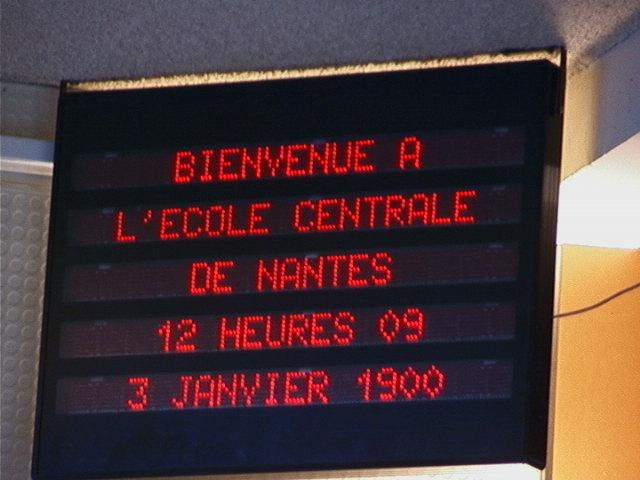
\includegraphics[width=10cm, height=8cm]{./images/bug10.jpg}
    \caption{Nouvelle Année}
\end{figure} 

\newpage
\subsection{A long terme}



\begin{table}[H]
\begin{tabular}{|p{3cm}|p{3cm}|p{3cm}|p{3cm}|}
\hline
\textit{\color{red}Prévention} & \textit{\color{red}Durabilité} & \textit{\color{red}Conscience} & \textit{\color{red}Collaboration} \\ \cline{1-4}
Le bug Y2K a souligné l'importance de la gestion proactive des risques technologiques, menant à l'adoption de cadres de gestion des risques plus robustes. & Le bug a encouragé l'adoption de pratiques de programmation durables et maintenables à long terme, avec un accent sur la gestion des données de date et de temps.& Sensibilisation à la Cybersécurité : Le bug a sensibilisé le public aux vulnérabilités des systèmes informatiques, soulignant l'importance de la cybersécurité et de la maintenance constante.&Coopération Internationale : La réponse mondiale a démontré l'importance de la coopération internationale pour relever les défis technologiques mondiaux.\\ \cline{1-4}
\end{tabular}
\caption{Tableau des Suites du BUG}
\end{table}

\begin{figure}[H]
    \centering
    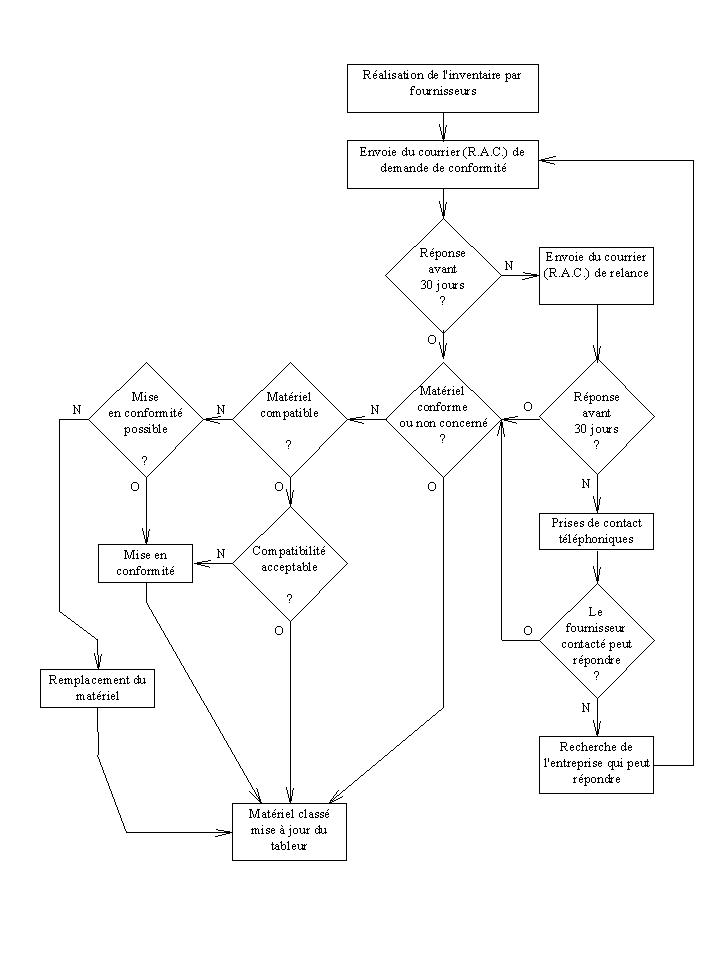
\includegraphics[width=10cm, height=8.5cm]{./images/shema.JPG}
    \caption{Schéma du remplacement ou modification des produit informatique d'un endroit}  
\end{figure}


\newpage
\begin{center}

\section{\textit{Conclusion}}


Le bug Y2K demeure un événement emblématique qui a laissé une empreinte indélébile sur notre approche des défis technologiques. Il continue d'influencer les pratiques de développement logiciel, la cybersécurité et la collaboration internationale, nous rappelant l'importance de l'anticipation, de la planification méticuleuse et du travail collaboratif dans un monde technologiquement dépendant.

\end{center}


\begin{center}
\textit{\textbf{\color{red}LES POINTS A RETENIR :}}
\end{center}
\begin{enumerate}
   \item \underline{\textbf{Origine du problème :}} Le bogue de l'an 2000, également appelé Y2K, est né de la programmation informatique qui utilisait souvent une convention à deux chiffres pour représenter les années (par exemple, "99" pour "1999").

    \item \underline{\textbf{Risque de dysfonctionnements :}} Lorsque l'année 2000 est arrivée, de nombreux systèmes informatiques ont été incapables de faire la distinction entre les années "00" (2000) et "99" (1900), ce qui a entraîné des erreurs et des dysfonctionnements.

    \item \underline{\textbf{Secteurs affectés :}} Le bogue de l'an 2000 a touché un large éventail de systèmes informatiques, notamment ceux utilisés dans les secteurs des finances, des transports, de la santé et de l'énergie.

    \item \underline{\textbf{Préparation et correction :}} Pour atténuer les risques, des efforts considérables ont été déployés pour identifier et corriger les systèmes affectés. Des millions de lignes de code ont été révisées et des tests ont été effectués pour garantir la stabilité des systèmes.

    \item \underline{\textbf{Coût financier :}} Le coût total des efforts de préparation et de correction du bogue de l'an 2000 a été estimé à des dizaines de milliards de dollars à l'échelle mondiale.

    \item \underline{\textbf{Impacts limités :}} Malgré les craintes initiales, le passage à l'an 2000 s'est déroulé relativement sans encombre, grâce aux mesures préventives prises par les entreprises et les gouvernements.

   \item \underline{\textbf{Leçons apprises :}} Le bogue de l'an 2000 a mis en lumière l'importance de la planification et de la gestion des risques en matière de technologie. Il a également souligné la nécessité de normes de codage claires et de pratiques de test rigoureuses pour assurer la fiabilité des systèmes informatiques à long terme.
\cite{vid}
\end{enumerate}




\newpage
\section{\textit{Bibliographie}}

\subsection*{Les Tableaux / Images}

\listoffigures
\listoftables



\bibliography{bibliographie}
\bibliographystyle{plain}




\end{document}